\documentclass[a4paper,12pt,french]{book}
\usepackage[T1]{fontenc}
\usepackage[utf8]{inputenc}
\usepackage{graphicx}
\usepackage{calc}

\usepackage[french]{babel}
\usepackage[european, straightvoltages, siunitx]{circuitikz}
\usetikzlibrary{babel}
\ctikzset{inductor=american}

\usepackage[version=4]{mhchem}

\usepackage{siunitx}

\usepackage{fancyhdr}
\pagestyle{fancy}

% Clear all header and footer fields
\fancyhf{}

% Define the header to include the chapter label
\fancyhead[LE,RO]{\leftmark $~$\rightmark} % Left pages (even): chapter, Right pages (odd): chapter

\newcommand{\e}[1]{\vspace{5mm}\noindent \textbf{\underline{#1}}}

\newcommand{\makeline}{\noindent\makebox[\linewidth]{\rule{\linewidth}{0.4pt}}}

\setcounter{secnumdepth}{-1}

\begin{document}
	
	

\author{Chams GHARIB}
\title{Colles de Physique-Chimie}
\date{2024-2025}

\frontmatter
\maketitle
\tableofcontents

\mainmatter
\chapter{MPSI}
\section{Semaine 01 (16/09-20/09) }


\e{Notions abordées :}
\begin{itemize}
	\item Analyse dimensionnelle.
	\item Circuits électriques dans l'ARQS.
\end{itemize}


\subsection{Questions de cours}

\begin{enumerate}
	\item Définir le courant électrique. Définir l'intensité du courant électrique.
	\item Définir la tension électrique.
	\item Décrire les conventions d'orientation des dipôles. Que valent la puissance reçues et fournies dans chaque cas ?
	\item Qu'est-ce que l'ARQS ? Quelles conséquences ?
	\item Démontrer la formule du pont diviseur de tension.
	\item Démontrer la formule du pont diviseur de courant.
\end{enumerate}

\subsection{Exercice 1 : Application des lois de Kirchoff}

Pour chaque circuit, donner les tensions $u$ et $u_1$ en fonction de $e$ ou bien les intensités $i$ et $i_1$ en fonction de $i_0$.

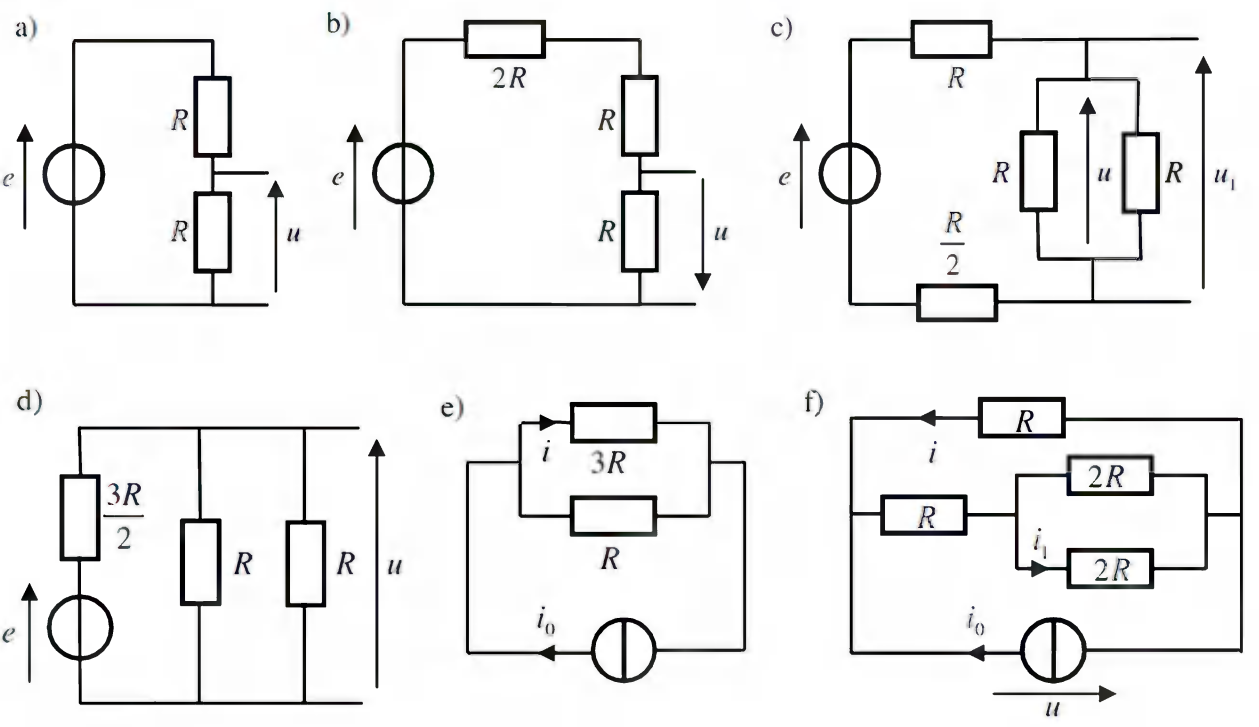
\includegraphics[width=\textwidth]{Images/exercicesKirchoff.png}

\subsection{Exercice 2}

\begin{minipage}[c]{\linewidth/2}
	\begin{circuitikz}
		%Circuit
		\draw (4, 0)
			to[short, i>=$I$] (2, 0)
			to[R, l=$R$] (0, 0)
			to[vsource, v_<=$e$] (0, -3)
			-- (4, -3);
		\draw (2, 0)
			to[R, l_=$R$, v^<=$U$] (2, -3);
	\end{circuitikz}
\end{minipage}%
\begin{minipage}[c]{\linewidth/2}
	On donne $R = \SI{10}{k\Omega}$.
	\begin{enumerate}
		\item Tracer la caractéristique du dipôle ci-contre.
		\item On ajoute une charge de résistance $R'=\SI{3}{k\Omega}$. Déterminer le point de fonctionnement de deux façons.
	\end{enumerate}
\end{minipage}

\subsection{Exercice 3 : Rendement d'un montage potentiométrique}

\begin{minipage}[c]{\linewidth/2}
	\begin{circuitikz}
		%Circuit
		\draw (0, 2)
		to[short, i>=$I$] (0, 3)
		--++(2, 0)
		to[R, l=$r_2$] ++(0, -2)
		to[R, l=$r_1$] ++(0, -2)
		--++(-2, 0)
		--++(0, 1)
		to[vsource, v=$E$] (0, 2);
		\draw (2, 1)
		to[short, i=$i_R$] ++(2, 0)
		to[R, l=$R$] ++(0, -2)
		--++(-2, 0);
	\end{circuitikz}
\end{minipage}%
\begin{minipage}[c]{\linewidth/2}
	Le rendement $\eta$ de ce diviseur de tension est le rapport $P_R$ de la puissance dissipée dans la résistance de charge $R$ à la puissance $P_E$ fournie par la source de tension $E$. Exprimer $\eta$ en fonction de $r_1$, $r_2$ et $R$.
	
	AN : $r_1 = \SI{750}{\Omega}$, $r_2=\SI{250}{\Omega}$, $R = \SI{80}{\Omega}$. Commentaire.
\end{minipage}

\subsection{Exercice 4 : Adaptation de puissance}

\begin{minipage}[c]{\linewidth/2}
	\begin{circuitikz}
		%Circuit
		\draw (0, 0)
		to[R, l=$R_0$] (3, 0)
		to[R, l=$R$] (3, -3)
		-- (0, -3)
		to[vsource, v=$E$] (0, 0);
	\end{circuitikz}
\end{minipage}%
\begin{minipage}[c]{\linewidth/2}
	Un générateur présente une tension à vide $E$ et une résistance interne $R_0$. On y branche une charge de résistance $R$. Pour quelle valeur de $R$ la puissance dissipée dans la résistance $R$ est elle maximale ? Que vaut alors cette puissance ?
\end{minipage}

\section{Semaine 02 (23/09-27/09) }


\e{Notions abordées :}
\begin{itemize}
	\item Circuits linéaires du premier ordre.
\end{itemize}

\subsection{Questions de cours}
\begin{enumerate}
	\item Relation entre la charge d'un condensateur et sa tension aux bornes.
	\item Relations entre intensité et tension pour un condensateur et une bobine.
	\item Continuité des grandeurs dans un circuit électrique.
	\item Établir l'expression de l'énergie stockée dans un condensateur/une bobine.
\end{enumerate}

\subsection{Exercice 1 : Résistance de fuite d'un condensateur}

Un condensateur réel présente des fuites de courants. Comment le modéliser ?

Il est inséré dans un circuit série comportant un générateur de f.é.m $E$, une résistance $r$ et un interrupteur $K$. On mesure la tension aux bornes du condensateur à l'aide d'un voltmètre idéal. On ferme $K$ et on attend que l'indication du voltmètre se stabilise. Puis on ouvre K en déclenchant au même instant un chronomètre. On constate que la tension indiquée par le voltmètre baisse de $10\%$ en un temps $T$.

On donne $E = \SI{1}{V}$, $r=\SI{10}{k\Omega}$, $T=\SI{1.0}{s}$ et $C=\SI{19}{\mu F}$.

\begin{enumerate}
	\item Exprimer la valeur $U$ vers laquelle la tension aux bornes du condensateur tend lorsque $K$ est fermé. En déduire une manière de déterminer $R_f$ (résistance de fuite).
	\item Montrer que la mesure du temps $T$ permet aussi de déterminer $R_f$. Commenter en relation avec l'une des hypothèses de l'énoncé.
\end{enumerate}

\subsection{Exercice 2 : Étude d'un circuit RL}

\begin{minipage}[c]{\linewidth/2}
	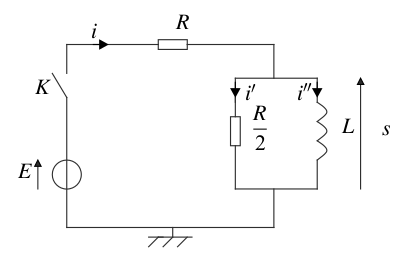
\includegraphics[width=\linewidth]{Images/mpsi_s02_ex02.png}
\end{minipage}%
\begin{minipage}[c]{\linewidth/2}
	À $t=0^-$, on ferme l'interrupteur $K$.
	\begin{enumerate}
		\item Donner $i$, $i'$, $i''$ et $s$ en $t=0^+$.
		\item Que vaut $s(t)$ lorsque $t$ tend vers l'infini.
		\item Établir l'équation différentielle vérifiée par $s(t)$.
		\item En déduire $s(t)$. En tracer l'allure.
		\item Exprimer le temps $t_0$ au bout duquel $s(t)$ a été divisé par $10$.
		\item On mesure $t_0=\SI{30}{\mu s}$ pour $R=\SI{1.0}{k\Omega}$. En déduire $L$.
	\end{enumerate}
\end{minipage}

\subsection{Exercice 3 : Rendement énergétique de la charge d'un condensateur}

On considère un circuit composé d'une résistance $R$ et d'un condensateur de capacité $C$ en série aux bornes duquel on place un générateur de tension idéal de f.é.m $E$ et un interrupteur $K$. À l'instant $t=0$, on ferme l'interrupteur $K$ et la tension $u_c$ aux bornes du condensateur est nulle.

\begin{enumerate}
	\item Établir l'équation différentielle vérifiée par $u_c$.
	\item Déterminer $u_c(t)$ et en tracer l'allure.
	\item Mêmes questions pour l'intensité du courant parcourant le circuit.
	\item Exprimer en fonction de $C$ et $E$ :
	\begin{itemize}
		\item L'énergie $\mathcal{E}_{elec}$ emmagasinée par le condensateur quand $t\rightarrow+\infty$.
		\item L'énergie $W_{Joule}$ dissipée par effet Joule dans la résistance entre $t=0$ et $t\rightarrow+\infty$.
		\item L'énergie $W_{gen}$ fournie par le générateur entre $t=0$ et $t\rightarrow+\infty$.
	\end{itemize}
	\item Donner une relation liant $\mathcal{E}_{elec}$, $W_{Joule}$ et $W_{gen}$ et proposer une interprétation physique de cette relation. Comment définir puis exprimer un rendement ?

\end{enumerate}
\section{Semaine 03 (30/09-04/10) }


\e{Notions abordées :}
\begin{itemize}
	\item Circuits linéaires du premier ordre (cf semaine précédente).
	\item Équilibre chimique.
\end{itemize}

\subsection{Questions de cours}
\begin{enumerate}
	\item Une mole de méthane réagit avec une mole de dioxygène selon une réaction de combustion. Déterminer la composition finale du système. (Équilibrer + Tableau d'avancement + Avancement final pour une réaction totale).
	\item Exprimer l'activité d'une espèce chimique dans un mélange. Préciser les hypothèses nécessaires.
	\item Exprimer le quotient réactionnel d'une réaction donnée et prévoir le sens d'évolution spontanée d'un système chimique.
\end{enumerate}

\subsection{Exercice 1 : Fluoration du dioxyde d'uranium}

Le dioxyde d'uranium solide réagit avec le fluorure d'hydrogène gazeux pour former du tétrafluorure d'uranium solide et de la vapeur d'eau. 

On maintient la température égale à $\SI{700}{K}$ et la pression totale à $\SI{1}{bar}$. La constante d'équilibre à $\SI{700}{K}$ est égale à $K^\circ = 6.8\times10^4$.

\begin{enumerate}
	\item Écrire la réaction.
	\item On part de $\SI{1.0}{mol}$ de dioxyde d'uranium et de $\SI{1.0}{mol}$ de fluorure d'hydrogène. Quelle sera la composition finale du système ?
	\item Même question en partant de $\SI{0.10}{mol}$ de dioxyde d'uranium et de $\SI{1.0}{mol}$ de fluorure d'hydrogène. Que remarque-t-on dans ce cas ?  
\end{enumerate}

\e{Réponses :}
\begin{enumerate}
	\item -
	\item $\xi = \SI{0.24}{mol}$.
	\item - 
\end{enumerate}

\subsection{Exercice 2 : Constante d'équilibre et quotient de réaction.}

Pour préparer industriellement du dihydrogène, on fait réagir en phase gazeuse du méthane avec de l'eau. La réaction produit également du monoxyde de carbone.

La réaction se déroule sous une pression totale constante $p_{tot} = \SI{10}{bar}$. La constante d'équilibre vaut $K^\circ = 15$. Initialement, le système contient $\SI{10}{mol}$ de méthane, $\SI{30}{mol}$ d'eau, $\SI{5}{mol}$ de monoxyde de carbone et $\SI{15}{mol}$ de dihydrogène. 

\begin{enumerate}
	\item Exprimer la constante d'équilibre en fonction des pressions partielles des constituants.
	\item Exprimer le quotient de réaction $Q$ en fonction de la quantité de matière de chacun des constituants et de la pression totale. Calculer $Q$ dans l'état initial.
	\item Le système est-il à l'équilibre thermodynamique ? Si non, dans quel sens se produira l'évolution ?
	\item Déterminer la composition du système à l'équilibre.
\end{enumerate}

\e{Réponses :}
\begin{enumerate}
	\item -
	\item $Q = 1.56$.
	\item -
	\item $\xi = \SI{3.6}{mol}$.
\end{enumerate}

\subsection{Exercice 3 : Utilisation du quotient de réaction.}

Un récipient de volume $V_0 = \SI{2.00}{L}$ contient initialement $\SI{0.500}{mol}$ de COBr$_2$ qui se décompose à une température de $\SI{346}{K}$ selon la réaction : $$\ce{COBr2_{(g)} = CO_{(g)} + Br2_{(g)}}$$.

\begin{enumerate}
	\item Déterminer la composition du système à l'équilibre sachant que la constante d'équilibre à $\SI{346}{K}$ vaut $K^\circ = 5.46$.
	\item Calculer le pourcentage de COBr$_2$ décomposé à cette température.
	\item L'équilibre précédent étant réalisé, on ajoute $\SI{2.00}{mol}$ de monoxyde de carbone. L'équilibre chimique est-il réalisé ? Si non, décrire l'évolution ultérieure du système.
\end{enumerate}

\e{Réponses :}
\begin{enumerate}
	\item $\xi = \SI{0.285}{mol}$.
	\item 57 \%.
	\item $Q = 43.2$, $\xi' = \SI{0.077}{mol}$.
\end{enumerate}
\section{Semaine 04 (07/10-11/10) }


\e{Notions abordées :}
\begin{itemize}
	\item Équilibre chimique (cf semaine précédente).
	\item Bases de l'optique géométrique.
\end{itemize}

\subsection{Questions de cours}
\begin{enumerate}
	\item Énoncer les lois de Snell-Descartes.
	\item Définir un rayon lumineux et un MTHI.
	\item Indice de réfraction ? Phénomène de réflexion totale ?
\end{enumerate}

\subsection{Exercice 1 : Réfractomètre de Pulrich}

\begin{minipage}[c]{\linewidth/2}
	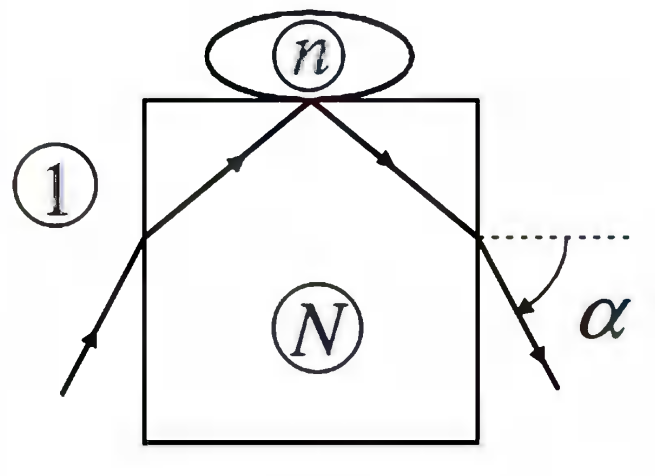
\includegraphics[width=\linewidth]{Images/mpsi_s04_ex01.png}
\end{minipage}%
\begin{minipage}[c]{\linewidth/2}
	Un réfractomètre de Pulrich est constitué d'un cube de verre d'indice $N$ connu sur lequel on a déposé une goutte d'un liquide d'indice $n$ inconnu. On observe un faisceau de rayons parallèles à la limite réfraction - réflexion totale et on mesure l'angle $\alpha$ correspondant. On donne $N=1.626$ et $\alpha=60$°.
\end{minipage} 

\begin{enumerate}
	\item Que vaut $n$ ?
	\item Quelles sont les valeurs mesurables de $n$ avec ce dispositif ?
\end{enumerate}

\e{Réponse} : $n = 1.376$

\subsection{Exercice 2}

\begin{minipage}[c]{\linewidth/2}
	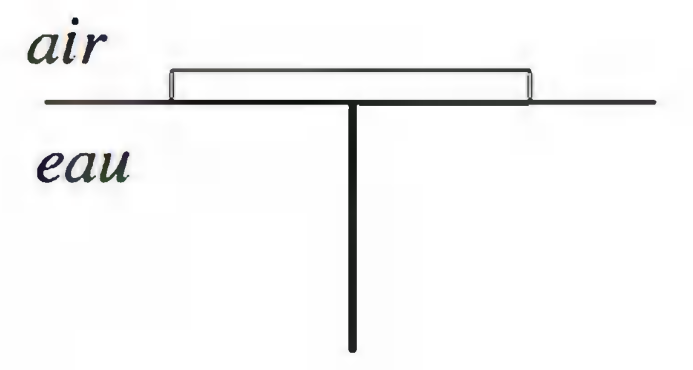
\includegraphics[width=\linewidth]{Images/mpsi_s04_ex02.png}
\end{minipage}%
\begin{minipage}[c]{\linewidth/2}
	Un disque en liège de diamètre $D = \SI{5}{cm}$ flotte sur l'eau. Il soutient une tige placée perpendiculairement en son centre. 
	
	Quelle est la longueur $h$ de la partie de la tige qu'un observateur dans l'air ne peut pas voir ?
\end{minipage}

\e{Réponse :} $h = \SI{2.1}{cm}$.

\subsection{Exercice 3 : Détection de pluie sur un pare-brise}

\begin{minipage}[c]{\linewidth/2}
	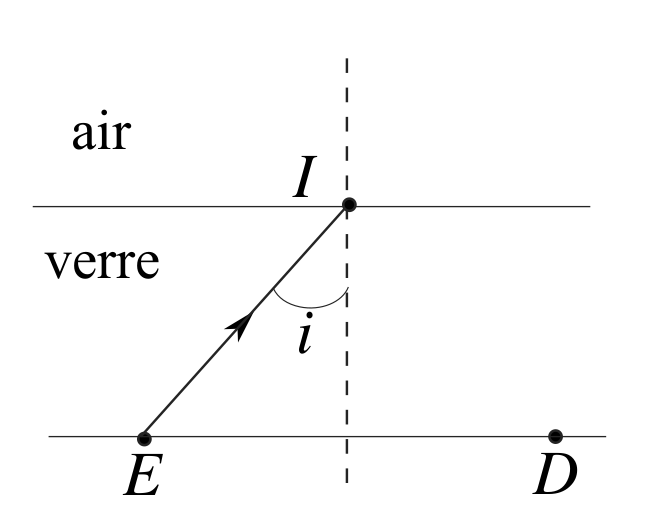
\includegraphics[width=\linewidth]{Images/mpsi_s04_ex03.png}
\end{minipage}%
\begin{minipage}[c]{\linewidth/2}
	On modélise un pare-brise par une lame de verre à faces parallèles, d'épaisseur $e = \SI{5}{mm}$, d'indice $n_v = 1.5$. Un fin pinceau lumineux issu d'un émetteur situé en $E$ arrive de l'intérieur du verre sur le dioptre verre/air en $I$ avec un angle d'incidence $i=60$°.
\end{minipage}

\begin{enumerate}
	\item Montrer que le flux lumineux revient intégralement sur le détecteur situé en $D$ et déterminer la distance $ED$.
	\item Comment ce dispositif permet-il de détecter un dépôt de pluie sur le pare-brise ? On supposera une épaisseur d'eau de $\SI{1}{mm}$.
\end{enumerate}

\e{Réponses :}
\begin{enumerate}
	\item $i_{lim} = 41.8$°.
	\item Distance au détecteur de $\SI{0.9}{cm}$.
\end{enumerate}


\section{Semaine 05 (14/10-18/10) }


\e{Notions abordées :}
\begin{itemize}
	\item Bases de l'optique géométrique (cf semaine précédente).
	\item Systèmes optiques.
\end{itemize}

\subsection{Questions de cours}

\textit{Cf exercices}

\subsection{Exercice 1 : Méthode de Bessel pour la focométrie}

On considère un objet transverse (AB) et un écran distants de $D$, ainsi qu'une lentille convergente de focale $f'$.

\begin{enumerate}
	\item Tracer les rayons dans le cas d'une image réelle.
	\item À quelle condition peut-on former l'image de l'objet sur l'écran ? Démonstration.
	\item Déterminer les positions de la lentille qui permettent d'obtenir une image sur l'écran. En déduire une méthode pour déterminer $f'$.
\end{enumerate}

\subsection{Exercice 2 : Microscope}

\begin{minipage}[c]{\linewidth/2}
	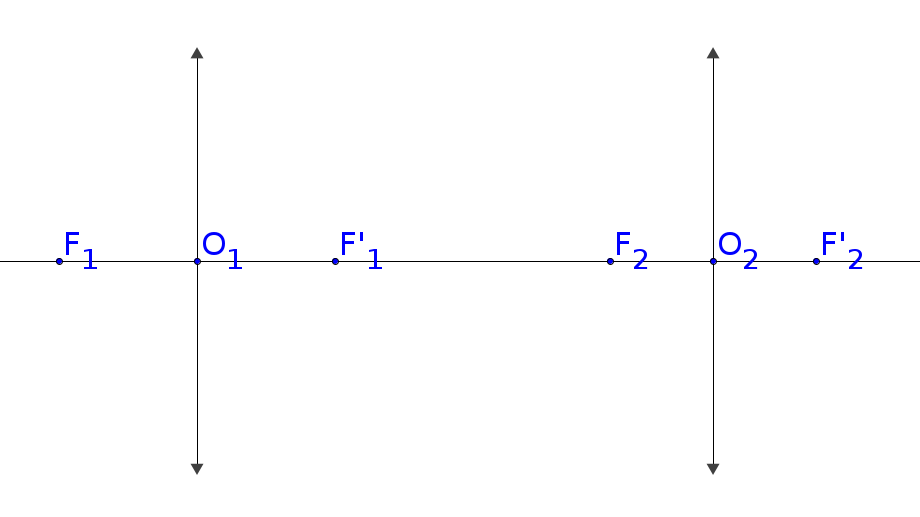
\includegraphics[width=\textwidth]{./Images/mpsi_s05_ex02.png}
\end{minipage}%
\begin{minipage}[c]{\linewidth/2}
	On donne $\overline{O_1O_2} = D_0 = \SI{75}{mm}$, $f'_1 = \SI{10}{mm}$ et $f'_2 = \SI{25}{mm}$.
\end{minipage}
 
\begin{enumerate}
	\item Que sont les conditions de Gauss et à quoi servent elles ?
	\item On pose $\Delta = \overline{F'_1F'_2}$. Exprimer $\Delta$ en fonction des données du problème. Calcul.
	\item On souhaite qu'un œil au repos voie l'image $A'B'$ de $AB$ par le système optique. Où est $A'B'$.
	\item Où doit alors être l'image intermédiaire $A_1B_1$ ?
	\item Exprimer la position de l'objet $AB$ en fonction de $f'_1$ et $\Delta$. Calcul.
	\item Étude du grossissement :
	\begin{enumerate}
		\item Quelle est la taille maximale de l'image que l'on peut avoir sur la rétine sans microscope ?
		\item Quelle est la taille de l'image sur la rétine avec microscope ?
		\item En déduire le "grossissement commercial" du microscope.
	\end{enumerate}
\end{enumerate}

\subsection{Exercice 3 : Lunette astronomique}

On souhaite observer Mars. Soit $\alpha$ le diamètre angulaire sous lequel elle est vue à l'œil nu. Pour cela on utilise un système optique composé de deux lentilles convergentes de focales respectives $f'_1=f'_{obj}$ et $f'_2=f'_{oc}$ (l'oculaire est du côté de l'œil, l'objectif est du côté de l'objet Mars).

\begin{enumerate}
	\item On utilise un système afocal. Définir afocal. En déduire la position relative des deux lentilles.
	\item Faire le tracé des rayons. L'image est-elle droite ou renversée ?
	\item Soit $\alpha'$ le diamètre angulaire en sortie du système optique. Exprimer le grossissement $G = \alpha'/\alpha$. Interpréter cette grandeur.
	\item \label{qprec} On veut augmenter le grossissement et renverser l'image. On interpose entre l'objectif et l'oculaire une troisième lentille convergente de focale $f'_3$. On déplace l'oculaire pour pouvoir observer l'image au repos. Quel couple de points cette nouvelle lentille doit elle conjuguer ?
	\item Faire le tracé des rayons.
	\item Soit $\gamma_3$ le grandissement de la nouvelle lentille associé au couple de points de la question \ref{qprec}. Exprimer $\overline{O_3F'_{obj}}$ en fonction de $\gamma_3$ et $f'_3$.
	\item Quel est le grossissement $G'$ de ce nouveau système optique. Le comparer à $G$ et conclure.
\end{enumerate}


\subsection{Exercice 4 : Stigmatisme d'une lame à faces parallèles}

Une lame à faces parallèles d'épaisseur $e$ est constituée d'un verre d'indice $n$. Elle est placée dans l'air. 

\begin{enumerate}
	\item Construire le cheminement d'un rayon arrivant sur le premier dioptre avec l'incidence $i$. Soit $r$ l'angle de réfraction. Le rayon transmis par la lame est-il dévié par rapport au rayon incident ? Comment appeler la modification subie ?
	\item On considère un objet ponctuel $A$ sur le rayon incident. Calculer la distance entre le prolongement du rayon incident et le rayon transmis en fonction de $e$, $i$ et $r$. 
	\item Rappeler ce qu'est le stigmatisme. Le système considéré est-il stigmatique ?
	\item On se place maintenant dans les conditions de Gauss. Montrer que le système est approximativement stigmatique et déterminer la relation de conjugaison donnant $\overline{AA'}$ en fonction de $n$ et $e$.
	\item Dans un parc aquatique, les aquariums ont une épaisseur de verre de $\SI{60}{cm}$. Situé à $\SI{20}{cm}$ de la vitre, un visiteur observe un requin marteau nageant à $\SI{1.0}{m}$ devant lui. À quelle distance semble-t-il être pour l'observateur ?
\end{enumerate}

\e{Réponse :} $\overline{R'A} = \SI{75.0}{cm}$.

\section{Semaine 06 (04/11-08/11) }


\e{Notions abordées :}
\begin{itemize}
	\item Systèmes optiques (cf semaine précédente).
	\item Cinétique chimique.
\end{itemize}

\subsection{Questions de cours}

\begin{enumerate}
	\item Définir la vitesse d'une réaction chimique. Quelle est son unité ?
	\item Qu'est ce que l'ordre d'une réaction chimique ? L'ordre partiel ? La constante de vitesse ?
	\item Donner la loi d'Arrhenius.
\end{enumerate}

\subsection{Exercice 1 : Décomposition de l'azométhane en phase gazeuse}

Dans un récipient de volume fixé $V$, on introduit à $\SI{600}{K}$ de l'azométhane \ce{CH3N2CH3_{(g)}}. Celui-ci se décompose en éthane et en diazote gazeux. 

L'évolution de la réaction est suivie par manométrie et une série de mesures a donné la pression partielle $p_A$ en azométhane : 

\begin{tabular}{|c|c|c|c|c|c|}
	\hline 
	$t$ ($10^3$ s) & $0$ & $1.00$ & $2.00$ & $3.00$ & $4.00$ \\ \hline
	$p_A$ ($10^{-2}$ mmHg) & $p_0 = 8.21$ & $5.74$ & $4.00$ & $2.80$ & $1.96$ \\ \hline
\end{tabular}

\begin{enumerate}
	\item Écrire l'équation bilan de la réaction.
	\item Vérifier que la réaction est d'ordre $1$ par rapport au réactif et calculer sa constante de vitesse.
\end{enumerate}

\e{Réponse :} $k = \SI{3.58e-4}{\per\second}$

\subsection{Exercice 2 : Temps de demi-réaction}

La réaction de décomposition totale du pentaoxyde de diazote \ce{N2O5} en dioxyde d'azote \ce{NO2} et dioxygène a lieu en phase gazeuse. L’expérience est menée dans un récipient de volume V constant, initialement vide, en amenant du pentaoxyde de diazote de manière à ce que la pression initiale soit $p_0$.

\begin{enumerate}
	\item On mesure la pression $p(t)$ au cours du temps. On veut évaluer la constante cinétique en mesurant le temps de demi-réaction. Quelle doit être la lecture de $p$ sur le manomètre pour ce temps ?
	\item Le tracé de la courbe $\ln{p(\ce{N2O5})}$ en fonction du temps est une droite. En déduire l'ordre de la réaction. Tracer l'allure de la pression en fonction du temps.
	\item Une première mesure réalisée à $\theta = \SI{150}{\celsius}$ permet de mesurer un temps de demi réaction $t_{1/2} = \SI{7.5}{s}$. Une seconde mesure réalisée à $\theta' = \SI{100}{\celsius}$ permet de mesurer un temps de demi-réaction $t'_{1/2} = \SI{7.0}{min}$. Calculer la constante de vitesse pour ces deux températures.
	\item Calculer l'énergie d'activation de la réaction.
\end{enumerate}

\e{Réponses :}
\begin{enumerate}
	\item $p_{1/2} = \frac{7}{4}p_0$.
	\item -
	\item $k = \SI{9.2e-2}{\per\second}$ et $k' = \SI{1.7e-3}{\per\second}$.
	\item $E_a = \SI{1.1e2}{\kilo\joule\per\mol}$.
\end{enumerate}

\subsection{Exercice 3 : Dismutation des ions hypochlorites}

En solution aqueuse, les ions hypochlorite \ce{ClO-} peuvent se dismuter selon la réaction totale $$\ce{ClO- = \frac{1}{3} ClO3- + \frac{2}{3}Cl-}$$.

La vitesse de la réaction $r$, définie comme la vitesse de disparition des ions hypochlorite \ce{ClO-} suit une loi cinétique de second ordre, dont la constante de vitesse est notée $k$.

On provoque cette réaction dans une solution contenant initialement des ions hypochlorite à la concentration $c_0 = \SI{0.10}{\mol\per\liter}$.

À $T = \SI{343}{K}$, la constante de vitesse de la solution est $k = \SI{3.1e-3}{\per\mol \deci \meter \cubed \per \second}$. 

L’énergie d’activation de cette réaction au voisinage des températures considérées ici est $E_a = \SI{47}{\kilo\joule\per\mol}$.

\begin{enumerate}
	\item Donner l’équation horaire de la concentration en ions hypochlorite.
	\item Au bout de combien de temps, noté $t_{30}$, aura-t-on obtenu la disparition de $30\%$ des ions hypochlorite ?
	\item Quel serait à $T' = \SI{363}{K}$ le temps $t_{30}'$ nécessaire pour obtenir le même taux d'avancement de $30 \%$ à partir de la même solution initiale ?
\end{enumerate}

\e{Réponses :}
\begin{enumerate}
	\item -
	\item $t_{30} = \SI{23}{min}$.
	\item $t_{30}' = \SI{9}{min}~\SI{20}{s}$.
\end{enumerate}


\section{Semaine 07 (11/11-15/11) }


\e{Notions abordées :}
\begin{itemize}
	\item Cinétique chimique (cf semaine précédente).
	\item Oscillateurs harmoniques.
\end{itemize}

\subsection{Questions de cours}

\begin{enumerate}
	\item Établir et reconnaître l'équation d'un circuit $LC$. La résoudre compte tenu des conditions initiales.
	\item Résoudre l'équation de l'oscillateur harmonique avec les conditions initiales $u(0)=3E$ et $\dot{u}(0)=4 \omega E$. Quelle est la phase à l'origine ?
	\item Dans le cadre du circuit $LC$ libre montrer la conservation et l'équipartition de l'énergie (conditions initiales arbitraires).
\end{enumerate}

\e{Exercices de chimie cf semaine précédente.}


\section{Semaine 08 (18/11-22/11) }


\e{Notions abordées :}
\begin{itemize}
	\item Oscillateur harmonique (cf semaine précédente).
	\item Oscillateur amorti.
\end{itemize}

\subsection{Questions de cours}

\begin{enumerate}
	\item Établir l'équation d'un circuit $RLC$ série.
	\item Donner l'équation de l'oscillateur amorti et ses solutions dans le cas général.
	\item Résoudre l'équation de l'oscillateur harmonique avec les conditions initiales $u(0)=3E$ et $\dot{u}(0)=4 \omega E$. Quelle est la phase à l'origine ?
\end{enumerate}

\subsection{Exercice 1 : Exemple de régime critique}

\begin{minipage}[c]{\linewidth/2}
	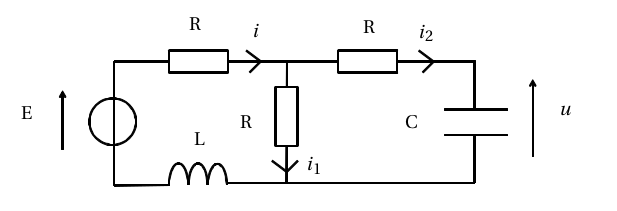
\includegraphics[width=\textwidth]{/home/chams/Documents/Travail/2024-2025/Colles/Images/mpsi_s08_ex01.png}
\end{minipage}%
\begin{minipage}[c]{\linewidth/2}
	Initialement le condensateur est déchargé et aucun courant ne traverse la bobine.
\end{minipage}

\begin{enumerate}
	\item Déterminer l'équation différentielle vérifiée par $u(t)$.
	\item Quelle est la relation entre $R$, $L$ et $C$ pour vérifier la condition de régime critique ? On suppose cette condition vérifiée dans la suite.
	\item Quelles sont les conditions initiales ? Déterminer également $u(\infty)$ et $i(\infty)$.
	\item Déterminer $u(t)$.
\end{enumerate}

\e{Réponses :}
\begin{enumerate}
	\item $u'' + 1/2(3R/L + 1/RC)u' + u/LC = E/2LC$
	\item $L = R^2 C$
	\item $u=0$, $u'=0$.
	\item $u(t) = E/2 - E/2(1+t/RC)e^{-t/RC}$
\end{enumerate}

\subsection{Exercice 2 : Étude d'un circuit à deux bobines}

\begin{minipage}[c]{\linewidth/2}
	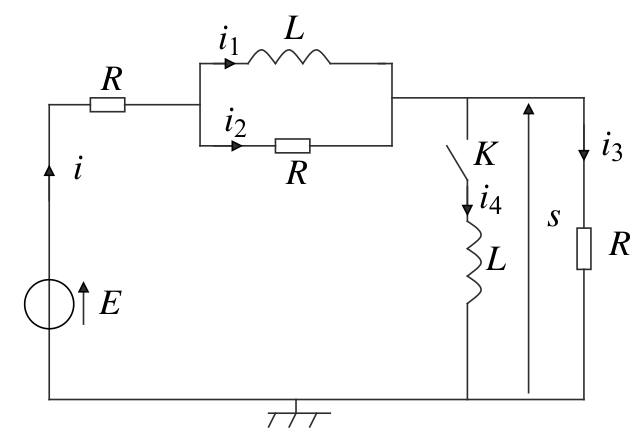
\includegraphics[width=\textwidth]{/home/chams/Documents/Travail/2024-2025/Colles/Images/mpsi_s08_ex02.png}
\end{minipage}%
\begin{minipage}[c]{\linewidth/2}
	À $t=0$, on ferme $K$
\end{minipage}

\begin{enumerate}
	\item Établir l'équation différentielle vérifiée par $s(t)$.
	\item Déterminer les conditions initiales pour $i$, $i_1$, $i_2$, $i_3$ et $i_4$. Déterminer également leurs valeurs pour $t\rightarrow+\infty$.
	\item Déterminer $s(t)$. 
\end{enumerate}

\e{Réponses :}
\begin{enumerate}
	\item $3s'' + 4R/L s' + (R/L)^2 s = 0$
	\item En $t=0^+$, $i_1=E/2R$, $i_3=E/2R$, $i=E/R$, $i_2=0$, $i_4=0$.
	\item $s(t) = \frac{E}{4} \left( \exp -\frac{R}{L}t +  \exp -\frac{R}{3L}t \right)$
\end{enumerate}


\subsection{Exercice 3 : Réponse à un échelon de tension d'un dipôle $RLC$ parallèle}

\begin{minipage}[c]{\linewidth/2}
	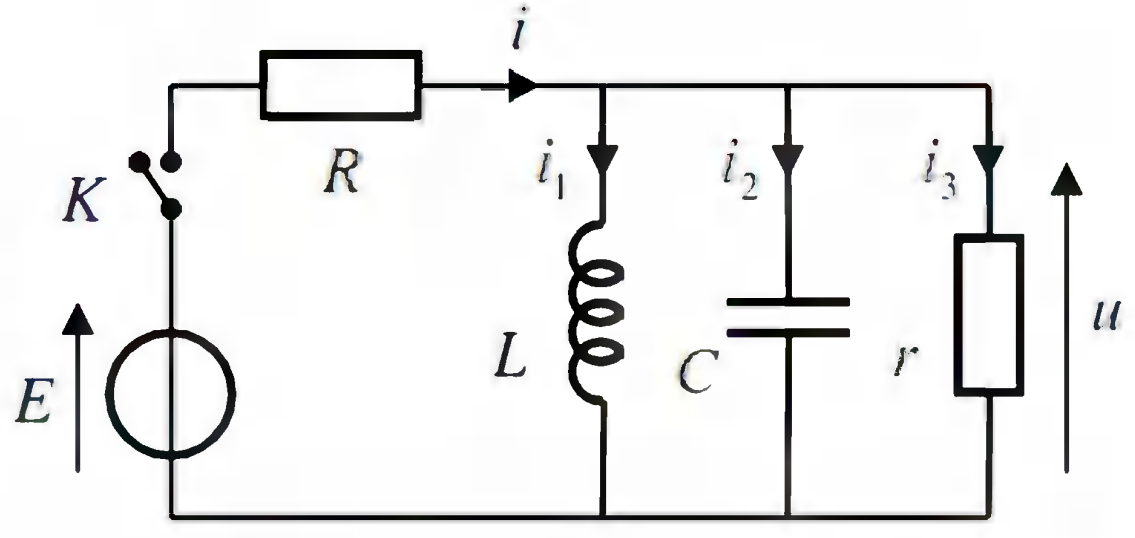
\includegraphics[width=\textwidth]{/home/chams/Documents/Travail/2024-2025/Colles/Images/mpsi_s08_ex03.png}
\end{minipage}%
\begin{minipage}[c]{\linewidth/2}
	Pour $t<0$, le condensateur est déchargé et la bobine idéale n'est parcourue par aucun courant. À $t=0$, on ferme $K$
\end{minipage}

\begin{enumerate}
	\item Établir l'équation différentielle vérifiée par $i_3$. La mettre sous forme canonique.
	\item Déterminer les conditions initiales. Déterminer également la valeur de $i_3$ pour $t\rightarrow+\infty$.
	\item Donner la relation entre $R$, $r$, $L$ et $C$ pour que le régime soit de type pseudopériodique et exprimer $i_3(t)$ dans ce cas.
\end{enumerate}

\e{Réponses :}
\begin{enumerate}
	\item $\omega_0 = \frac{1}{\sqrt{LC}}$, $\frac{\omega_0}{Q} = \frac{R + r}{RrC}$.
	\item En $t=0^+$, $u=0$, $i_1=0$, $i_3=0$, $i=E/R$, $i_2=E/R$. En $t\rightarrow+\infty$, $u=0$, $i=i_1=E/R$, $i_2=i_3=0$
	\item $\frac{2rR}{R+r} > \sqrt{\frac{L}{C}}$
\end{enumerate}


\section{Semaine 09 (25/11-29/11) }


\e{Notions abordées :}
\begin{itemize}
	\item Oscillateurs.
	\item Propagation d'un signal
\end{itemize}

\subsection{Questions de cours}

\begin{enumerate}
	\item Citer quelques exemples d'ondes. Préciser leurs caractéristiques (polarisation, milieu de propagation, ordre de grandeur de la célérité).
	\item Qu'est-ce qu'une onde progressive ?
	\item Qu'est ce qu'une onde progressive sinusoïdale ?
\end{enumerate}

\e{Exercices : cf semaine précédente}


\chapter{MPI}

\section{Semaine 02 (23/09-27/09) }


\e{Notions abordées :}
\begin{itemize}
	\item Révisions de MPSI en électronique.
	\item Filtrage d'un signal périodique.
\end{itemize}

\subsection{Exercice 1}

\begin{minipage}[c]{\linewidth/3}
	\begin{circuitikz}
		%Circuit
		\draw (0, 0) 
		to[R, l=$R$] (3, 0)
		to [L, l=$L$, v<=$v_s$] ++ (0, -2)
		-- (0, -2)
		to [open, v=$v_e$] (0, 0);
	\end{circuitikz}
\end{minipage}%
\begin{minipage}[c]{\linewidth/2}
	On donne $R = \SI{1.0}{k\Omega}$ et $L = \SI{10}{mH}$.
	\begin{enumerate}
		\item Quel type de filtre ce circuit permet-il de réaliser ?
		\item Déterminer sa fonction de transfert.
		\item Déterminer les pentes des asymptotes en gain BF et HF.
		\item $v_e$ s'écrit comme somme de trois harmoniques de même amplitude, de même phase à l'origine et de fréquences respectives $f_1 = \SI{100}{Hz}$, $f_2 = \SI{1}{kHz}$ et $f_3 = \SI{100}{kHz}$. Écrire $v_e$ puis $v_s$.
		\item $v_e$ est maintenant un triangle de fréquence \SI{60}{Hz}. Quelle est la forme de $v_s$ ?
	\end{enumerate}
\end{minipage}

\subsection{Exercice 2}

\begin{minipage}[c]{\linewidth/2}
	\begin{circuitikz}
		%Circuit
		\draw (0, 0) 
		to[R, l=$R$] (3, 0)
		to[C, l=$C$] ++(2, 0)
		to [L, l=$L$, v<=$v_s$] ++ (0, -2)
		-- (0, -2)
		to [open, v=$v_e$] (0, 0);
	\end{circuitikz}
\end{minipage}%
\begin{minipage}[c]{\linewidth/2}
	\begin{enumerate}
		\item Quel type de filtre ce circuit permet-il de réaliser ?
		\item Déterminer sa fonction de transfert.
		\item Déterminer les pentes des asymptotes en gain BF et HF. Tracer le diagramme de Bode asymptotique.
		\item $v_e$ s'écrit comme somme de trois harmoniques de même amplitude, de même phase à l'origine et de fréquences respectives $f_1 = \SI{100}{Hz}$, $f_2 = \SI{1}{kHz}$ et $f_3 = \SI{100}{kHz}$. Écrire $v_e$ puis $v_s$.
		\item Ce filtre peut-il avoir un comportement dérivateur ? Intégrateur ?
	\end{enumerate}
\end{minipage}

\subsection{Exercice 3}

\begin{minipage}[c]{\linewidth/2}
	\begin{circuitikz}
		%Circuit
		\draw (0, 0) 
		to[R, l=$R$] (2, 0)
		to[C, l=$C$] ++(2, 0)
		to [R, l=$R$] ++ (0, -2)
		-- (0, -2)
		to [open, v=$v_e$] (0, 0);
		\draw (4, 0)
		-- (6, 0)
		to [C, l=$C$, v<=$v_s$] ++ (0, -2)
		-- (4, -2)
		;
	\end{circuitikz}
\end{minipage}%
\begin{minipage}[c]{\linewidth/2}
	On donne $R = \SI{1.0}{k\Omega}$ et $C = \SI{500}{nF}$.
	\begin{enumerate}
		\item Quel type de filtre ce circuit permet-il de réaliser ?
		\item Déterminer sa fonction de transfert.
		\item Déterminer la bande passante. Définir le facteur de qualité.
		\item $v_e$ s'écrit comme somme de trois harmoniques de même amplitude, de même phase à l'origine et de fréquences respectives $f_1 = \SI{100}{Hz}$, $f_2 = \SI{1}{kHz}$ et $f_3 = \SI{100}{kHz}$. Écrire $v_e$ puis $v_s$.
	\end{enumerate}
\end{minipage}


\section{Semaine 03 (30/09-04/10) }


\e{Notions abordées :}
\begin{itemize}
	\item Électronique de MPSI.
	\item Filtrage d'un signal périodique.
	\item Numérisation.
	\item Portes logiques.
\end{itemize}

\subsection{Exercice 1 : Intégration d'un créneau par un filtre passe bande}

Une tension créneau est injectée dans un filtre passe-bande non inverseur d'ordre 2, de pulsation de résonance $\omega_0$, de facteur de qualité $Q$ et de gain maximum $G_0$. La pulsation $\omega$ de la tension créneau est supposée grande devant $\omega_0$.

\begin{enumerate}
	\item Écrire la fonction de transfert du filtre.
	\item Montrer que ce filtre se comporte vis-à-vis du créneau d'entrée comme un intégrateur.
	\item Écrire l'équation différentielle reliant la tension d'entrée $v_e(t)$ et la tension de sortie $v_s(t)$ de l'intégrateur. Qu'obtient-on précisément en sortie du filtre ? Comment seraient modifiés les résultats si on ajoutait une tension continue au créneau à l'entrée ?
\end{enumerate}

\subsection{Exercice 2 : Shannon comme au cinéma}

Au cinéma, lorsqu'on regarde les roues d'une voiture qui démarre, on les voit d'abord tourner dans le sens réel puis elles semblent tourner à l'envers. Expliquer d'où provient cette illusion. Qu'observe-t-on en visionnant le film lorsque les roues de la voiture tournent à $f_1=\SI{1200}{tours/min}$ ? Et à $f_2 = \SI{1680}{tours/min}$.


\section{Semaine 04 (07/10-11/10) }


\e{Notions abordées :}
\begin{itemize}
	\item Électrocinétique.
	\item Mécanique de MPSI.
\end{itemize}

\subsection{Exercice 1 : Système à deux ressorts}

On considère une masse $m$ astreinte à se déplacer sur un axe horizontal $(Ox)$ et fixée à une paroi à gauche et une à droite par deux ressorts identiques $(k, l_0)$. Les parois sont distantes de $L$.

\begin{enumerate}
	\item Appliquer le principe fondamental de la dynamique à la masse $m$.
	\item En déduire la position d'équilibre $x_e$.
	\item Étudier les petites oscillations autour de la position d'équilibre.
	\item On envisage l'existence d'un frottement fluide d'intensité proportionnelle à la vitesse via une constante $\beta$. Établir l'équation différentielle du mouvement. Pour quelles valeurs de $\beta$ la masse $m$ oscille-t-elle ?
	\item Comment choisir $\beta$ pour un retour le plus rapide à la position d'équilibre. Quel est le temps caractéristique d'amortissement ?
\end{enumerate}

\subsection{Exercice 2 : Frottement et facteur de qualité}

On considère un ressort horizontal de constante de raideur $k$ et de longueur à vide $l_0$. Une extrémité du ressort est fixe et l'autre attachée à un mobile de masse $m$. Le mobile subit une force de frottement fluide proportionnelle à sa vitesse via une constante $\beta$.

\begin{enumerate}
	\item Déterminer l'équation différentielle du mouvement. Introduire une pulsation propre et un facteur de qualité.
	\item Résoudre l'équation différentielle. Simplifier l'expression dans le cas $Q \gg 1$.
	\item En déduire que $Q$ est une bonne approximation du nombre d'oscillations avant le retour à l'équilibre.
	\item On considère maintenant l'énergie mécanique relative perdue sur une pseudo-période. L'exprimer en fonction de $Q$. 
	\item On considère maintenant un opérateur qui impose une force $\vec{F(t)} = m A \cos{\omega t} \vec{e_x}$. Déterminer la fonction de transfert du système et interpréter $Q$ d'une nouvelle façon.
\end{enumerate}

\subsection{Exercice 3 : Mouvement autour d'une position d'équilibre}

Soit un point matériel de masse $m$ astreint à se déplacer selon un axe $(Ox)$ et d'énergie potentielle $E_p(x) = \frac{-a}{x^2} + \frac{b}{x^3}$ avec $a, b > 0$.

\begin{enumerate}
	\item Montrer en général qu'une position d'équilibre correspond à un extremum local d'énergie potentiel. À quelle condition une position d'équilibre est-elle stable ? instable ?
	\item Tracer le profil d'énergie potentiel.
	\item Déterminer la ou les position(s) d'équilibre ainsi que leur stabilité.
	\item Étudier les petites oscillations autour de la position d'équilibre stable.
	\item Déterminer, dans le cas d'une énergie potentielle générale, l'expression de la pulsation des petites oscillations.
\end{enumerate}

\section{Semaine 04 (14/10-18/10) }


\e{Notions abordées :}
\begin{itemize}
	\item Mécanique de MPSI (forces centrales).
	\item Dynamique en référentiel non galiléen.
\end{itemize}

\subsection{Exercice 1 : Force en $1/r^4$}

On considère un point matériel de masse $m$ soumis à la force $\vec{F} = \frac{-K}{r^4} \vec{e}_r$, avec $K>0$.

\begin{enumerate}
	\item Montrer que le mouvement est plan et qu'il vérifie la loi des aires.
	\item Définir une énergie potentielle effective et la tracer.
	\item Discuter graphiquement les trajectoires possibles. Justifier. Existe-t-il une trajectoire circulaire ?
\end{enumerate}

\subsection{Exercice 2 : Satellite géostationnaire}

\begin{enumerate}
	\item Définir un satellite géostationnaire et déterminer son orbite. Justifier.
	\item Quel travail faut il fournir pour l'élever en altitude de $\SI{50}{km}$ ? 
	\item L'essence à une énergie spécifique de $\SI{13.1}{kWh/kg}$ et une masse volumique de $\SI{745}{\kilogram\per\cubic\meter}$. En déduire le volume de carburant nécessaire pour effectuer la manœuvre.
\end{enumerate}

\e{Réponses :}
\begin{enumerate}
	\item $\SI{42e3}{km}$
	\item $\SI{5.7e6}{J}$
	\item $\SI{0.13}{kg}$ et $\SI{0.16}{\liter}$.
\end{enumerate}

\subsection{Exercice 3 : Chute d'un satellite dans l'atmosphère}

\begin{enumerate}
	\item Un satellite est en orbite circulaire autour de la Terre. Montrer qu'il existe une relation simple entre $E_c$ et $E_p$. Exprimer l'énergie mécanique en fonction de $r$.
	\item Comment évolue la vitesse d'un satellite freiné par l'atmosphère ?
	\item Son altitude est $h=\SI{180}{km}$ et la force de frottement a pour norme $\beta m v^2 / h$.
	\begin{enumerate}
		\item Préciser l'unité de $\beta$.
		\item Déterminer la variation d'altitude $\Delta h$ après une révolution. On proposera les hypothèses appropriées.
	\end{enumerate}
\end{enumerate}

\e{Réponse :} $\Delta h = \SI{-28.3}{m}$.

\subsection{Exercice 4 : Pendule pesant dans une voiture accélérée}

Une tige homogène de longueur $l$ et de masse totale $m$ est accrochée en un point $A$ du plafond d'une voiture. La voiture est en translation rectiligne d'accélération $a$ par rapport au référentiel terrestre supposé galiléen. 

Le moment d'inertie de la tige par rapport au point $A$ est $J = \frac{1}{3}m l ^2$. On admet que le point d'application de la force d'inertie d'entraînement est le centre d'inertie de la tige.

\begin{enumerate}
	\item Déterminer l'angle d'équilibre du pendule dans le référentiel de la voiture.
	\item Déterminer la période $T$ des petites oscillations du pendule autour de la position d'équilibre.
\end{enumerate}

\subsection{Exercice 5 : Limite de Roche}

\begin{minipage}[c]{\linewidth/2}
	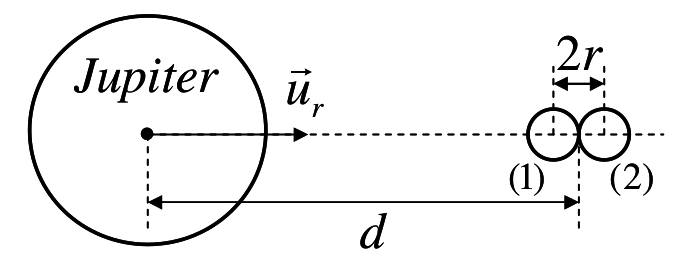
\includegraphics[width=\linewidth]{Images/mp_s04_ex02.png}
\end{minipage}%
\begin{minipage}[c]{\linewidth/2}
	On cherche à déterminer la distance en dessous de laquelle une comète s'approchant de Jupiter se sépare en plusieurs morceaux sous l'effet des forces de marée dues à Jupiter.
	
	On modélise la comète par deux sphères identiques de masses $m$ et de rayon $r$, alignées comme sur le dessin. On suppose que la comète est en orbite circulaire de rayon $d$ autour de Jupiter.
\end{minipage} 

\begin{enumerate}
	\item Montrer que le mouvement du centre d'inertie de la comète est uniforme. Quelle est la nature du mouvement du référentiel barycentrique de la comète par rapport au référentiel de Jupiter ?
	\item Soit $\vec{R}$ la réaction de la sphère $(1)$ sur la sphère $(2)$. Dans le référentiel de la comète, appliquer le PFD à une des deux sphères.
	\item À quelle condition le contact entre les sphères est-il rompu ? Déterminer, sachant que $r \ll d$, la distance limite $d_{lim}$ en dessous de laquelle il ne peut exister de comètes.
\end{enumerate}

\e{Données :} $M_J = \SI{1.9e27}{kg}$, $R_J = \SI{7.1e4}{km}$ et masse volumique de la comète $\rho_c = \SI{1.0e3}{\kilogram\per\cubic\metre}$.

\e{Réponse :} $d_{lim} = \SI{1.8e5}{km}$.

\subsection{Exercice 6 : Usure d'une ligne de TGV}

Un train grande vitesse se dirige vers le sud, depuis Paris (latitude $48.8$°). On considère son mouvement dans le référentiel terrestre non galiléen. Montrer qu'apparaît une réaction horizontale de la voie sur le train. La comparer à la réaction verticale. 


\subsection{Exercice 7 : Impesanteur}

Existe-t-il un endroit où $\vec{g} = \vec{0}$ ? Commenter la valeur numérique obtenue.

\e{Réponse :} $\SI{42e3}{km}$
\section{Semaine 06 (04/11-08/11) }


\e{Notions abordées :}
\begin{itemize}
	\item Mécanique de MPSI.
	\item Dynamique en référentiel non galiléen.
	\item Lois du frottement de Coulomb.
\end{itemize}

\subsection{Exercice 1 : Glissement d'une caisse dans un camion}

\begin{minipage}[c]{\linewidth/2}
	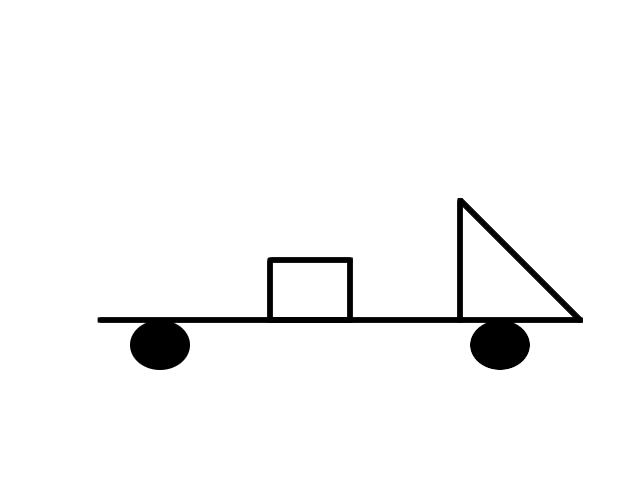
\includegraphics{/home/chams/Documents/Travail/2024-2025/Colles/Images/mp_s05_ex01.png}
\end{minipage}%
\begin{minipage}[c]{\linewidth/2}
	Le camion accélère avec l'accélération constante $a$.
	\begin{enumerate}
		\item À quelle condition le glissement commence-t-il ?
		\item Au bout de combien de temps la caisse atteint-elle le rebord ?
		\item Quelle distance parcourt-elle après être tombée ?
		\item La caisse glisse-t-elle ou bascule-t-elle lors de l'accélération ?
	\end{enumerate}
\end{minipage}

\subsection{Exercice 2 : Cube sur un plan incliné}

Un cube repose sur un plan incliné d'un angle $\alpha$. On augmente $\alpha$ très lentement.

\begin{enumerate}
	\item À quelle condition le glissement commence-t-il ?
	\item À quelle condition le cube bascule-t-il ?
	\item Qu'est ce qui arrive en premier ? On donne le coefficient de frottement bois-bois $f = 0.4$.
\end{enumerate}

\subsection{Exercice 3 : Glissement et liaison avec une corde}

\begin{minipage}[c]{\linewidth/2}
	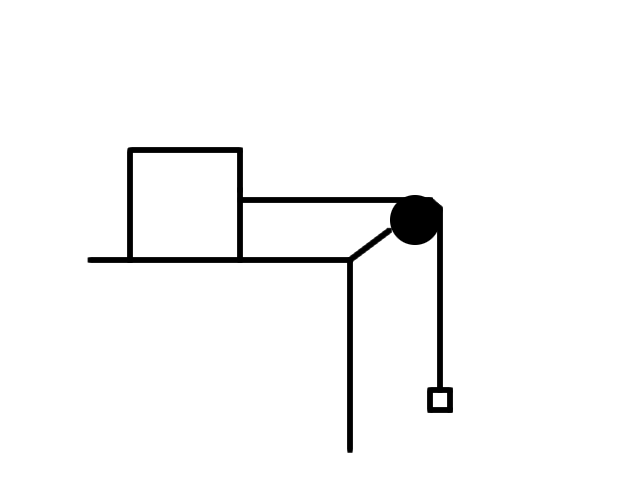
\includegraphics{/home/chams/Documents/Travail/2024-2025/Colles/Images/mp_s05_ex03.png}
\end{minipage}%
\begin{minipage}[c]{\linewidth/2}
	Deux caisses sont liées par une corde qui passe par une poulie. On prend en compte le frottement de la grosse caisse sur la surface. En précisant les hypothèses utilisées, déterminer l'altitude de la caisse suspendue en fonction du temps.
\end{minipage}
\section{Semaine 07 (11/11-15/11) }


\e{Notions abordées :}
\begin{itemize}
	\item Transformations chimiques d'un système.
	\item Acides et bases, réactions acide-base.
\end{itemize}

\subsection{Questions de cours :}
\begin{enumerate}
	\item Une mole de méthane réagit avec une mole de dioxygène selon une réaction de combustion. Déterminer la composition finale du système.
	\item Exprimer l'activité d'une espèce chimique pure, en phase condensée ou très diluée en solution aqueuse.
	\item Exprimer le quotient réactionnel d'une réaction donnée et prévoir le sens d'évolution spontanée d'un système chimique.
\end{enumerate}

\subsection{Exercice 1 : Fluoration du dioxyde d'uranium}

Le dioxyde d'uranium solide réagit avec le fluorure d'hydrogène gazeux pour former du tétrafluorure d'uranium solide et de la vapeur d'eau. 

On maintient la température égale à $\SI{700}{K}$ et la pression totale à $\SI{1}{bar}$. La constante d'équilibre à $\SI{700}{K}$ est égale à $K^\circ = 6.8\times10^4$.

\begin{enumerate}
	\item Écrire la réaction.
	\item On part de $\SI{1.0}{mol}$ de dioxyde d'uranium et de $\SI{1.0}{mol}$ de fluorure d'hydrogène. Quelle sera la composition finale du système ?
	\item Même question en partant de $\SI{0.10}{mol}$ de dioxyde d'uranium et de $\SI{1.0}{mol}$ de fluorure d'hydrogène. Que remarque-t-on dans ce cas ?  
\end{enumerate}

\e{Réponses :}
\begin{enumerate}
	\item -
	\item $\xi = \SI{0.24}{mol}$.
	\item - 
\end{enumerate}

\subsection{Exercice 2 : Constante d'équilibre et quotient de réaction.}

Pour préparer industriellement du dihydrogène, on fait réagir en phase gazeuse du méthane avec de l'eau. La réaction produit également du monoxyde de carbone.

La réaction se déroule sous une pression totale constante $p_{tot} = \SI{10}{bar}$. La constante d'équilibre vaut $K^\circ = 15$. Initialement, le système contient $\SI{10}{mol}$ de méthane, $\SI{30}{mol}$ d'eau, $\SI{5}{mol}$ de monoxyde de carbone et $\SI{15}{mol}$ de dihydrogène. 

\begin{enumerate}
	\item Exprimer la constante d'équilibre en fonction des pressions partielles des constituants.
	\item Exprimer le quotient de réaction $Q$ en fonction de la quantité de matière de chacun des constituants et de la pression totale. Calculer $Q$ dans l'état initial.
	\item Le système est-il à l'équilibre thermodynamique ? Si non, dans quel sens se produira l'évolution ?
	\item Déterminer la composition du système à l'équilibre.
\end{enumerate}

\e{Réponses :}
\begin{enumerate}
	\item -
	\item $Q = 1.56$.
	\item -
	\item $\xi = \SI{3.6}{mol}$.
\end{enumerate}

\subsection{Exercice 3 : Utilisation du quotient de réaction.}

Un récipient de volume $V_0 = \SI{2.00}{L}$ contient initialement $\SI{0.500}{mol}$ de COBr$_2$ qui se décompose à une température de $\SI{346}{K}$ selon la réaction : $$\ce{COBr2_{(g)} = CO_{(g)} + Br2_{(g)}}$$.

\begin{enumerate}
	\item Déterminer la composition du système à l'équilibre sachant que la constante d'équilibre à $\SI{346}{K}$ vaut $K^\circ = 5.46$.
	\item Calculer le pourcentage de COBr$_2$ décomposé à cette température.
	\item L'équilibre précédent étant réalisé, on ajoute $\SI{2.00}{mol}$ de monoxyde de carbone. L'équilibre chimique est-il réalisé ? Si non, décrire l'évolution ultérieure du système.
\end{enumerate}

\e{Réponses :}
\begin{enumerate}
	\item $\xi = \SI{0.285}{mol}$.
	\item 57 \%.
	\item $Q = 43.2$, $\xi' = \SI{0.077}{mol}$.
\end{enumerate}
\section{Semaine 08 (18/11-22/11) }


\e{Notions abordées :}
\begin{itemize}
	\item Transformations chimiques d'un système.
	\item Acides et bases, réactions acide-base.
	\item Réaction d'oxydoréduction et piles.
	\item Dosages.
\end{itemize}

\subsection{Questions de cours}

\begin{enumerate}
	\item Réaliser le schéma d'une pile. 
	\item Écrire une réaction d'oxydoréduction entre l'ion cuivre au degré d'oxydation $2$ et l'argent solide.
	\item Écrire l'équation d'une réaction acide-base et déterminer la valeur de sa constante thermodynamique d'équilibre en fonction des $pKa$ des couples mis en jeu.
\end{enumerate}

\subsection{Exercice 1 : Vitamine C}

La vitamine C, aussi appelée acide ascorbique, est un diacide noté $AscH_2$.

\begin{enumerate}
	\item Dresser le diagramme de prédominance des espèces acido-basiques issues de l'acide ascorbique en fonction du $pH$ de la solution.
	\item On dissout dans l'eau un comprimé contenant $\SI{500}{mg}$ d'acide ascorbique dans une fiole jaugée de volume $V = \SI{200}{mL}$. Déterminer l'état d'équilibre de la solution obtenue.
	\item La vitamine C existe aussi en comprimé tamponné, réalisée en mélangeant l'acide ascorbique $AscH_2$ et de l'ascorbate de sodium $AscHNa$. Un comprimé de vitamine C tamponnée de masse $m$ en principe actif (acide ascorbique sous ses deux formes, diacide et monoacide) est dissous dans $V'=\SI{100}{mL}$ d'eau distillée. La solution obtenue a un $pH$ égal à $4.4$. Déterminer la masse d'acide ascorbique et la masse d'ascorbate de sodium contenues dans ce cachet. On prendra $m=\SI{500}{mg}$ pour les applications numériques.
\end{enumerate}

\e{Données :} 
\begin{itemize}
	\item Les deux $pKa$ associés à l'espèce étudiée sont $4.2$ et $11.6$.
	\item $M(AscH_2) = \SI{176}{\gram \per \mol}$, $M(AscHNa) = \SI{198}{\gram \per \mol}$.
	\item S'il y a plusieurs réactions possibles, on se concentrera sur celle dont la constante thermodynamique est la plus élevée (réaction prépondérante).
\end{itemize} 

\e{Réponses :}
\begin{enumerate}
	\item -
	\item $[AscH_2] = \SI{1.4e-2}{\mol\per\liter}$, $[AscH_-] = [H_3O^+] = \SI{9.4e-4}{\mol\per\liter}$
	\item $m_a = \SI{1.9e2}{mg}$, $m_b=\SI{3.4e2}{mg}$.
\end{enumerate}

\subsection{Exercice 2 : Titrage du dioxyde de soufre dans le vin}

La concentration en masse de dioxyde de soufre dans un vin blanc ne doit pas excéder $\SI{210}{\milli\gram\per\liter}$. Pour vérifier la conformité de la concentration en dioxyde de soufre d'un vin blanc, on utilise une solution titrante de concentration $C_1 = \SI{7.80e-3}{\mol\per\liter}$ en diiode. Dans un erlenmeyer, on verse un volume $V_2 = \SI{25.0}{mL}$ de vin blanc. On ajoute $\SI{2}{mL}$ d'acide sulfurique pour acidifier le milieu. Lors du titrage du vin blanc, l'équivalence est obtenue après avoir versé un volume $V_E = \SI{6.1}{mL}$ de solution titrante. La réaction support du titrage s'écrit $$\ce{SO2(aq) + I2(aq) + 2H2O(l) \rightarrow SO4^{2-}(aq) + 2I-(aq) + 4H+(aq)}$$

Ce vin est il conforme à la législation ?

\e{Donnée :} $M(SO_2) = \SI{64.1}{g\per\mol}$

\e{Réponse :} $\SI{120}{mg/L} < \SI{210}{mg/L}$.

\subsection{Exercice 3 : Pile à combustible}

Dans certaines piles à combustible, on utilise le dihydrogène comme combustible et le dioxygène comme comburant. 

\begin{enumerate}
	\item Écrire la réaction de combustion du dihydrogène par le dioxygène.
	\item Cette réaction est en fait l'association de deux demi-équations d'oxydoréduction mettant en jeu les couples \ce{H^+/H2_{(g)}} et \ce{O2_{(g)}/H2O}. Écrire les demi-équations d'oxydoréduction.
	\item Les deux demi-réactions ont lieu sur deux électrodes. Indiquer la réaction cathodique et la réaction anodique.
	\item Donner l'expression du potentiel d'oxydoréduction pour les deux couples.
	\item Exprimer la constante d'équilibre $K^o$ en fonction des potentiels standards des couples. Calculer sa valeur. Commenter.
\end{enumerate}

\e{Données :} $E^o(H^+, H_2) = 0.00~V$, $E^o(O_2, H_2O) = 1.23~V$.
\section{Semaine 09 (25/11-29/11) }


\e{Notions abordées :}
\begin{itemize}
	\item Transformations chimiques d'un système.
	\item Acides et bases, réactions acide-base.
	\item Réaction d'oxydoréduction et piles.
	\item Dosages.
\end{itemize}

\subsection{Questions de cours}

\begin{enumerate}
	\item Réaliser le schéma d'une pile. 
	\item Écrire une réaction d'oxydoréduction entre l'ion cuivre au degré d'oxydation $2$ et l'argent solide.
	\item Écrire l'équation d'une réaction acide-base et déterminer la valeur de sa constante thermodynamique d'équilibre en fonction des $pKa$ des couples mis en jeu.
\end{enumerate}

\e{Exercices : Cf semaine précédente}

\chapter{MP}
\section{Semaine 01 (16/09-20/09) }


\e{Notions abordées :}
\begin{itemize}
	\item Révisions de MPSI en électronique.
	\item Filtrage d'un signal périodique.
	\item Traitement numérique du signal.
\end{itemize}

\subsection{Exercice 1}

\begin{minipage}[c]{\linewidth/3}
	\begin{circuitikz}
		%Circuit
		\draw (0, 0) 
			to[R, l=$R$] (3, 0)
			to [L, l=$L$, v<=$v_s$] ++ (0, -2)
			-- (0, -2)
			to [open, v=$v_e$] (0, 0);
	\end{circuitikz}
\end{minipage}%
\begin{minipage}[c]{\linewidth/2}
	On donne $R = \SI{1.0}{k\Omega}$ et $L = \SI{10}{mH}$.
	\begin{enumerate}
		\item Quel type de filtre ce circuit permet-il de réaliser ?
		\item Déterminer sa fonction de transfert.
		\item Déterminer les pentes des asymptotes en gain BF et HF.
		\item $v_e$ s'écrit comme somme de trois harmoniques de même amplitude, de même phase à l'origine et de fréquences respectives $f_1 = \SI{100}{Hz}$, $f_2 = \SI{1}{kHz}$ et $f_3 = \SI{100}{kHz}$. Écrire $v_e$ puis $v_s$.
		\item $v_e$ est maintenant un triangle de fréquence \SI{60}{Hz}. Quelle est la forme de $v_s$ ?
	\end{enumerate}
\end{minipage}

\subsection{Exercice 2}

\begin{minipage}[c]{\linewidth/2}
	\begin{circuitikz}
		%Circuit
		\draw (0, 0) 
		to[R, l=$R$] (3, 0)
		to[C, l=$C$] ++(2, 0)
		to [L, l=$L$, v<=$v_s$] ++ (0, -2)
		-- (0, -2)
		to [open, v=$v_e$] (0, 0);
	\end{circuitikz}
\end{minipage}%
\begin{minipage}[c]{\linewidth/2}
	\begin{enumerate}
		\item Quel type de filtre ce circuit permet-il de réaliser ?
		\item Déterminer sa fonction de transfert.
		\item Déterminer les pentes des asymptotes en gain BF et HF. Tracer le diagramme de Bode asymptotique.
		\item $v_e$ s'écrit comme somme de trois harmoniques de même amplitude, de même phase à l'origine et de fréquences respectives $f_1 = \SI{100}{Hz}$, $f_2 = \SI{1}{kHz}$ et $f_3 = \SI{100}{kHz}$. Écrire $v_e$ puis $v_s$.
		\item Ce filtre peut-il avoir un comportement dérivateur ? Intégrateur ?
	\end{enumerate}
\end{minipage}

\subsection{Exercice 3}

\begin{minipage}[c]{\linewidth/2}
	\begin{circuitikz}
		%Circuit
		\draw (0, 0) 
			to[R, l=$R$] (2, 0)
			to[C, l=$C$] ++(2, 0)
			to [R, l=$R$] ++ (0, -2)
			-- (0, -2)
			to [open, v=$v_e$] (0, 0);
		\draw (4, 0)
			-- (6, 0)
			to [C, l=$C$, v<=$v_s$] ++ (0, -2)
			-- (4, -2)
			;
	\end{circuitikz}
\end{minipage}%
\begin{minipage}[c]{\linewidth/2}
	On donne $R = \SI{1.0}{k\Omega}$ et $C = \SI{500}{nF}$.
	\begin{enumerate}
		\item Quel type de filtre ce circuit permet-il de réaliser ?
		\item Déterminer sa fonction de transfert.
		\item Déterminer la bande passante. Définir le facteur de qualité.
		\item $v_e$ s'écrit comme somme de trois harmoniques de même amplitude, de même phase à l'origine et de fréquences respectives $f_1 = \SI{100}{Hz}$, $f_2 = \SI{1}{kHz}$ et $f_3 = \SI{100}{kHz}$. Écrire $v_e$ puis $v_s$.
	\end{enumerate}
\end{minipage}
\section{Semaine 02 (23/09-27/09) }


\e{Notions abordées :}
\begin{itemize}
	\item Mécanique du point.
	\item Traitement numérique du signal.
\end{itemize}

\subsection{Exercice 1}

\begin{enumerate}
	\item Définir un satellite géostationnaire et calculer son altitude.
	\item Quel travail faut il fournir pour augmenter son altitude de $\SI{50}{km}$.
\end{enumerate}

\subsection{Exercice 2}

On considère un point matériel astreint à se déplacer autour d'un anneau en rotation autour d'un diamètre, à $\omega$ constante.

Positions d'équilibre ? Stabilité ?

\subsection{Exercice 3}

On cherche à graver sur un $CD$ une musique. Toutefois, il existe un signal parasite à $f_p = \SI{42.1}{kHz}$. 

\begin{enumerate}
	\item Échantillonnage sur 16 bits. Quelle est la taille du fichier si la durée vaut $74$ minutes.
	\item Le critère de Shannon est il vérifié ? Conséquence ?
	\item Comment résoudre ce problème ?
\end{enumerate}


\subsection{Exercice 4}

Décrire le mouvement d'une particule chargée dans un champ magnétique statique uniforme.

\section{Semaine 03 (30/09-04/10) }

\e{Notions abordées :}
\begin{itemize}
	\item Traitement numérique du signal.
	\item Mécanique de MPSI.
	\item Dynamique en référentiel non galiléen.
\end{itemize}

\subsection{Exercice 1}

Une tige rigide est en rotation uniforme autour de son axe à la pulsation $\omega$. Un mobile M est lié par un fil au point O situé sur l'axe à l'altitude $h$. 

\begin{enumerate}
	\item Démontrer la loi de composition des accélérations pour un référentiel en rotation uniforme.
	\item Déterminer l'angle $\alpha_0$ d'équilibre du mobile.
	\item Étudier la stabilité de la position d'équilibre.
\end{enumerate}

\subsection{Exercice 2}

Un électron et un proton de même énergie cinétique sont plongés dans un champ magnétique uniforme, orthogonal à leur vitesse initiale.

\begin{enumerate}
	\item Décrire qualitativement les trajectoires.
	\item Comparer :
	\begin{itemize}
		\item Leur vitesse.
		\item Le rayon de leur trajectoire.
		\item Leur période.
	\end{itemize}
	\item Calculer la force centrifuge subie par l'électron.
\end{enumerate}

\subsection{Exercice 3}

Un mobile $M$ coulisse sans frottement  sur un axe horizontal $(Ox)$ dans un train qui accélère avec une accélération $A\vec{u_x}$, le point $O$ étant fixé à l'arrière du wagon. Entre $O$ et $M$ on place un ressort $(k, l_0)$. À $t=0$, $x=l_0$ et la vitesse de $M$ dans le référentiel du train est nulle.

\begin{enumerate}
	\item Démontrer la loi de composition des accélérations dans un référentiel uniformément accéléré.
	\item Établir $x(t)$.
\end{enumerate}




\section{Semaine 04 (07/10-11/10) }

\e{Notions abordées :}
\begin{itemize}
	\item Mécanique de MPSI (forces centrales et dynamique du solide).
	\item Dynamique en référentiel non galiléen.
\end{itemize}

\subsection{Exercice 1 : Pendule pesant dans une voiture accélérée}

Une tige homogène de longueur $l$ et de masse totale $m$ est accrochée en un point $A$ du plafond d'une voiture. La voiture est en translation rectiligne d'accélération $a$ par rapport au référentiel terrestre supposé galiléen. 

Le moment d'inertie de la tige par rapport au point $A$ est $J = \frac{1}{3}m l ^2$. On admet que le point d'application de la force d'inertie d'entraînement est le centre d'inertie de la tige.

\begin{enumerate}
	\item Déterminer l'angle d'équilibre du pendule dans le référentiel de la voiture.
	\item Déterminer la période $T$ des petites oscillations du pendule autour de la position d'équilibre.
\end{enumerate}

\subsection{Exercice 2 : Limite de Roche}

\begin{minipage}[c]{\linewidth/2}
	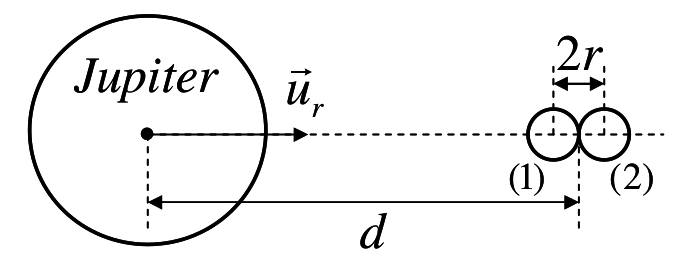
\includegraphics[width=\linewidth]{Images/mp_s04_ex02.png}
\end{minipage}%
\begin{minipage}[c]{\linewidth/2}
	On cherche à déterminer la distance en dessous de laquelle une comète s'approchant de Jupiter se sépare en plusieurs morceaux sous l'effet des forces de marée dues à Jupiter.
	
	On modélise la comète par deux sphères identiques de masses $m$ et de rayon $r$, alignées comme sur le dessin. On suppose que la comète est en orbite circulaire de rayon $d$ autour de Jupiter.
\end{minipage} 

\begin{enumerate}
	\item Montrer que le mouvement du centre d'inertie de la comète est uniforme. Quelle est la nature du mouvement du référentiel de la comète par rapport au référentiel de Jupiter ?
	\item Soit $\vec{R}$ la réaction de la sphère $(1)$ sur la sphère $(2)$. Dans le référentiel de la comète, appliquer le PFD à une des deux sphères.
	\item À quelle condition le contact entre les sphères est-il rompu ? Déterminer, sachant que $r \ll d$, la distance limite $d_{lim}$ en dessous de laquelle il ne peut exister de comètes.
\end{enumerate}

\e{Données :} $M_J = \SI{1.9e27}{kg}$, $R_J = \SI{7.1e4}{km}$ et masse volumique de la comète $\rho_c = \SI{1.0e3}{\kilogram\per\cubic\metre}$.

\e{Réponse :} $d_{lim} = \SI{1.8e5}{km}$.

\subsection{Exercice 3 : Usure d'une ligne de TGV}

Un train grande vitesse se dirige vers le sud, depuis Paris (latitude $48.8$°). On considère son mouvement dans le référentiel terrestre non galiléen. Montrer qu'apparaît une réaction horizontale de la voie sur le train. La comparer à la réaction verticale. 




\section{Semaine 05 (14/10-18/10) }

\e{Notions abordées :}
\begin{itemize}
	\item Mécanique de MPSI (forces centrales et dynamique du solide).
	\item Dynamique en référentiel non galiléen.
	\item Lois du frottement solide.
\end{itemize}

\subsection{Exercice 1 : Glissement d'une caisse dans un camion}

\begin{minipage}[c]{\linewidth/2}
	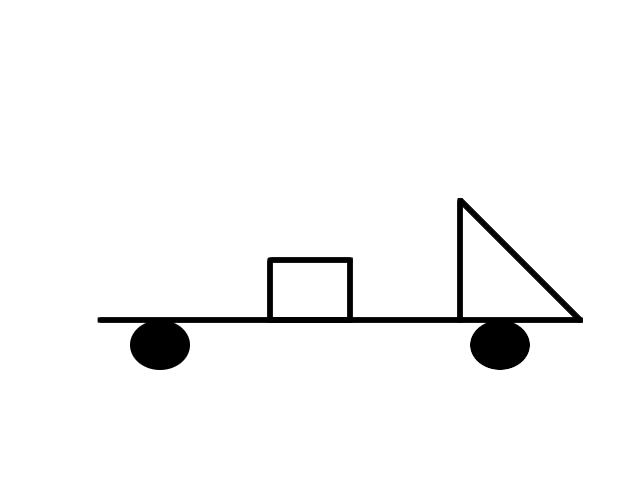
\includegraphics{/home/chams/Documents/Travail/2024-2025/Colles/Images/mp_s05_ex01.png}
\end{minipage}%
\begin{minipage}[c]{\linewidth/2}
	Le camion accélère avec l'accélération constante $a$.
	\begin{enumerate}
		\item À quelle condition le glissement commence-t-il ?
		\item Au bout de combien de temps la caisse atteint-elle le rebord ?
		\item Quelle distance parcourt-elle après être tombée ?
		\item La caisse glisse-t-elle ou bascule-t-elle lors de l'accélération ?
	\end{enumerate}
\end{minipage}

\subsection{Exercice 2 : Cube sur un plan incliné}

Un cube repose sur un plan incliné d'un angle $\alpha$. On augmente $\alpha$ très lentement.

\begin{enumerate}
	\item À quelle condition le glissement commence-t-il ?
	\item À quelle condition le cube bascule-t-il ?
	\item Qu'est ce qui arrive en premier ? On donne le coefficient de frottement bois-bois $f = 0.4$.
\end{enumerate}

\subsection{Exercice 3 : Glissement et liaison avec une corde}

\begin{minipage}[c]{\linewidth/2}
	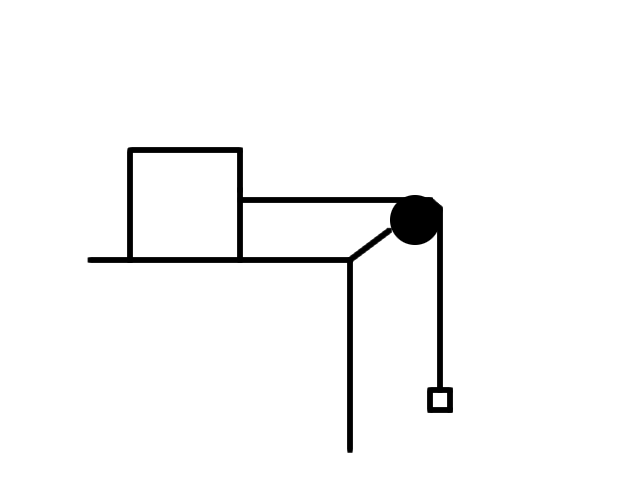
\includegraphics{/home/chams/Documents/Travail/2024-2025/Colles/Images/mp_s05_ex03.png}
\end{minipage}%
\begin{minipage}[c]{\linewidth/2}
	Deux caisses sont liées par une corde qui passe par une poulie. On prend en compte le frottement de la grosse caisse sur la surface. En précisant les hypothèses utilisées, déterminer l'altitude de la caisse suspendue en fonction du temps.
\end{minipage}



\section{Semaine 06 (04/11-08/11) }

\e{Notions abordées :}
\begin{itemize}
	\item Particules dans un $\vec{E}, \vec{B}$ statique (MPSI).
	\item Électrostatique :
	\begin{itemize}
		\item Distributions de charges et de courants.
		\item Symétries et invariances.
		\item Loi de Coulomb.
		\item Théorème de Gauss.
		\item Analogie gravitationnelle.
	\end{itemize}
\end{itemize}

\subsection{Exercice 1 : Condensateur cylindrique}

Deux cylindres métalliques $\mathcal{C}_1$ et $\mathcal{C}_2$ de même axe $(Oz)$, de même hauteur $h$ et de rayon $R_1$ et $R_2 > R_1$ portent des charges réparties uniformément en surface. On note $\sigma_1$ la densité surfacique de charge de $\mathcal{C}_1$.

\begin{enumerate}
	\item Quelle est la charge portée par $\mathcal{C}_2$ ? En déduire sa densité surfacique de charges.
	\item Déterminer la capacité $C$ de ce condensateur cylindrique. 
	\item Dans quel cas retrouve-t-on la capacité d'un condensateur plan ?
\end{enumerate}

\e{Réponse :} $C = \frac{2 \pi \epsilon_0 h}{\ln{R_2/R_1}}$

\subsection{Exercice 2 : Condensateur sphérique}

Deux sphères métalliques $\mathcal{S}_1$ et $\mathcal{S}_2$ de même centre $O$ et de rayons $R_1$ et $R_2 > R_1$ portent des charges réparties uniformément en surface. On note $\sigma_1$ la densité surfacique de charge de $\mathcal{S}_1$.

\begin{enumerate}
	\item Quelle est la charge portée par $\mathcal{S}_2$ ? En déduire sa densité surfacique de charges.
	\item Déterminer la capacité $C$ de ce condensateur sphérique.
	\item Dans quel cas retrouve-t-on la capacité d'un condensateur plan ?
\end{enumerate}

\e{Réponse :} $C = \frac{4 \pi \epsilon_0}{\frac{1}{R_1}-\frac{1}{R_2}}.$

\subsection{Exercice 3 : Rayon classique de l'électron}

L’électron de charge $-e$ est modélisé par une sphère $\mathcal{S}$ de centre $O$ et de rayon $R$ uniformément chargée dans son volume.

\begin{enumerate}
	\item Déterminer le champ électrique généré par l'électron.
	\item Évaluer l'énergie électrique $U_e$ d'un électron isolé liée à la seule présence du champ électrostatique qu'il crée.
	\item En assimilant cette énergie à l'énergie de repos $E=mc^2$ prévue par la relativité, déterminer le rayon $R_e$ de l'électron. Commentaire.
\end{enumerate}

\e{Réponse :} $R_e = \frac{3e^2}{20 \pi \epsilon_0 m_e c^2} = \SI{1.7e-15}{\meter}$
\section{Semaine 07 (11/11-15/11) }

\e{Notions abordées :}
\begin{itemize}
	\item Particules chargées dans un champ statique (MPSI).
	\item Chimie : Architecture de la matière (Atomistique, cristallographie).
	\item Chimie : Cinétique chimique (MPSI).
	\item Magnétostatique (Cours seulement).
\end{itemize}

\subsection{Questions de cours :}
\begin{enumerate}
	\item Champ créé par un fil infini parcouru par un courant $I$.
	\item Champ magnétique créé par un conducteur cylindrique infini parcouru par un courant uniforme.
	\item Champ créé par un solénoïde infini.
\end{enumerate}

\subsection{Exercice 1 : Décomposition de l'azométhane en phase gazeuse}

Dans un récipient de volume fixé $V$, on introduit à $\SI{600}{K}$ de l'azométhane \ce{CH3N2CH3_{(g)}}. Celui-ci se décompose en éthane et en diazote gazeux. 

L'évolution de la réaction est suivie par manométrie et une série de mesures a donné la pression partielle $p_A$ en azométhane : 

\begin{tabular}{|c|c|c|c|c|c|}
	\hline 
	$t$ ($10^3$ s) & $0$ & $1.00$ & $2.00$ & $3.00$ & $4.00$ \\ \hline
	$p_A$ ($10^{-2}$ mmHg) & $p_0 = 8.21$ & $5.74$ & $4.00$ & $2.80$ & $1.96$ \\ \hline
\end{tabular}

\begin{enumerate}
	\item Écrire l'équation bilan de la réaction.
	\item Vérifier que la réaction est d'ordre $1$ par rapport au réactif et calculer sa constante de vitesse.
\end{enumerate}

\e{Réponse :} $k = \SI{3.58e-4}{\per\second}$

\subsection{Exercice 2 : Temps de demi-réaction}

La réaction de décomposition totale du pentaoxyde de diazote \ce{N2O5} en dioxyde d'azote \ce{NO2} et dioxygène a lieu en phase gazeuse. L’expérience est menée dans un récipient de volume V constant, initialement vide, en amenant du pentaoxyde de diazote de manière à ce que la pression initiale soit $p_0$.

\begin{enumerate}
	\item On mesure la pression $p(t)$ au cours du temps. On veut évaluer la constante cinétique en mesurant le temps de demi-réaction. Quelle doit être la lecture de $p$ sur le manomètre pour ce temps ?
	\item Le tracé de la courbe $\ln{p(\ce{N2O5})}$ en fonction du temps est une droite. En déduire l'ordre de la réaction. Tracer l'allure de la pression en fonction du temps.
	\item Une première mesure réalisée à $\theta = \SI{150}{\celsius}$ permet de mesurer un temps de demi réaction $t_{1/2} = \SI{7.5}{s}$. Une seconde mesure réalisée à $\theta' = \SI{100}{\celsius}$ permet de mesurer un temps de demi-réaction $t'_{1/2} = \SI{7.0}{min}$. Calculer la constante de vitesse pour ces deux températures.
	\item Calculer l'énergie d'activation de la réaction.
\end{enumerate}

\e{Réponses :}
\begin{enumerate}
	\item $p_{1/2} = \frac{7}{4}p_0$.
	\item -
	\item $k = \SI{9.2e-2}{\per\second}$ et $k' = \SI{1.7e-3}{\per\second}$.
	\item $E_a = \SI{1.1e2}{\kilo\joule\per\mol}$.
\end{enumerate}

\subsection{Exercice 3 : Dismutation des ions hypochlorites}

En solution aqueuse, les ions hypochlorite \ce{ClO-} peuvent se dismuter selon la réaction totale $$\ce{ClO- = \frac{1}{3} ClO3- + \frac{2}{3}Cl-}$$.

La vitesse de la réaction $r$, définie comme la vitesse de disparition des ions hypochlorite \ce{ClO-} suit une loi cinétique de second ordre, dont la constante de vitesse est notée $k$.

On provoque cette réaction dans une solution contenant initialement des ions hypochlorite à la concentration $c_0 = \SI{0.10}{\mol\per\liter}$.

À $T = \SI{343}{K}$, la constante de vitesse de la solution est $k = \SI{3.1e-3}{\per\mol \deci \meter \cubed \per \second}$. 

L’énergie d’activation de cette réaction au voisinage des températures considérées ici est $E_a = \SI{47}{\kilo\joule\per\mol}$.

\begin{enumerate}
	\item Donner l’équation horaire de la concentration en ions hypochlorite.
	\item Au bout de combien de temps, noté $t_{30}$, aura-t-on obtenu la disparition de $30\%$ des ions hypochlorite ?
	\item Quel serait à $T' = \SI{363}{K}$ le temps $t_{30}'$ nécessaire pour obtenir le même taux d'avancement de $30 \%$ à partir de la même solution initiale ?
\end{enumerate}

\e{Réponses :}
\begin{enumerate}
	\item -
	\item $t_{30} = \SI{23}{min}$.
	\item $t_{30}' = \SI{9}{min}~\SI{20}{s}$.
\end{enumerate}
\section{Semaine 08 (18/11-22/11) }

\e{Notions abordées :}
\begin{itemize}
	\item Magnétostatique.
	\item Dipôle magnétostatique (cours seulement).
\end{itemize}

\subsection{Exercice 1 : Bobine torique}

On considère une bobine torique de rayon moyen $R$, comportant $N$ spires, de section carrée de côté $a$ et parcourue par un courant $I$. Déterminer le champ magnétique produit en tout point de l'espace. Comparer avec le champ magnétique du solénoïde infini.

\subsection{Exercice 2 : Caractéristiques d'un câble coaxial}

Un câble coaxial est constitué de deux cylindres conducteurs de rayons $R_1$ et $R_2 > R_1$ sur lesquels circulent, en surface, des courants d'intensité $I$ et de sens opposés.

\begin{enumerate}
	\item Déterminer le champ magnétique.
	\item La densité volumique d'énergie magnétique est donnée par $U_m = \frac{\vec{B}^2}{2 \mu_0}$. En déduire l'inductance linéique du câble coaxial.
	\item Les deux cylindres portent également des charges opposées. Reprendre les calculs pour le champ électrique. En déduire la capacité par unité de longueur.
	\item Quelle relation simple trouve-t-on entre l'inductance et la capacité ?
\end{enumerate}

\subsection{Exercice 3 : Équilibre d'une tige dans un champ non uniforme}

Une tige $[OA]$ de masse $m$ et de longueur $L$ est en rotation autour de l'axe $(Ox)$ horizontal. Son moment d'inertie est $J = \frac{1}{3} m L^2$. Elle est parcourue par un courant d'intensité $i$ dirigée de $O$ vers $A$. Son inclinaison par rapport à la verticale est mesurée par l'angle $\theta$. Un fil rectiligne d'axe vertical $(Oz)$ est parcouru par un courant de même intensité $i$ dirigée vers le haut. À l'équilibre de la tige, donner l'expression de $i$ en fonction de $\theta$, $L$, $m$ et $g$. 


\subsection{Exercice 4 : Action mécanique d'un fil sur un autre fil parallèle}

Deux fils rectilignes infinis parallèles sont distants de $d = \SI{1.0}{m}$. Ils sont parcourus par des courants de même intensité $I$ et de même sens. La force subie par un tronçon de longueur $L = \SI{1.0}{m}$ d’un des fils est égale $\SI{2.0e-7}{N}$.

Déterminer la valeur de $I$.

\section{Semaine 09 (25/11-29/11) }

\e{Notions abordées :}
\begin{itemize}
	\item Induction (révisions de MPSI) (priorité).
	\item Magnétostatique.
	\item Dipôles électro- et magnétostatiques.
\end{itemize}

\subsection{Exercice 1 : Double rails de Laplace}

Deux barres parallèles conductrices, de résistance $R$, sont posées à l'horizontale sur deux rails parallèles et conducteurs, séparés d'une distance $l$. L'une des barres est animée d'une vitesse $\vec{V}$. L'ensemble baigne dans un champ magnétique vertical homogène et stationnaire $\vec{B}$. 

\begin{enumerate}
	\item On suppose la vitesse $\vec{V}$ constante. Déterminer le mouvement de l'autre barre, d'abord qualitativement, puis quantitativement.
	\item Étudier le cas du régime sinusoïdal forcé.
\end{enumerate}

\subsection{Exercice 2 : Inductances propres et mutuelles}

\begin{enumerate}
	\item Rappeler la définitions des inductances propres et mutuelles. À quoi ces grandeurs nous servent-elles ?
	\item Calculer l'inductance propre d'un solénoïde de longueur $l$, de section $S$, comportant $N$ spires, et supposé suffisamment long pour négliger les effets de bords. Application numérique pour une bobine de TP.
	\item Exprimer l'énergie magnétique stockée dans la bobine. Retrouver l'expression de la densité volumique d'énergie magnétique.
	\item On considère un petit solénoïde à l'intérieur d'un gros solénoïde, les deux partageant le même axe. Déterminer l'inductance mutuelle.
\end{enumerate}

\e{Réponses :}
\begin{enumerate}
	\item -
	\item $L = \mu_0 \frac{N^2 S}{l}$
	\item -
	\item $M = \mu_0 \frac{N_1 N_2}{l_1}S_1$
\end{enumerate}

\subsection{Exercice 3 : Induction par un aimant mobile}

Une spire circulaire d'axe $(Oz)$, de rayon $a$ et de résistance $R$ est immobile. Sur son axe, on rapproche à vitesse $\vec{V} = V \vec{e_z}$ constante un petit aimant assimilé à un dipôle magnétique de moment $\vec{\mathcal{M}} = \mathcal{M}\vec{e_z}$.

\begin{enumerate}
	\item Prévoir le sens du courant $i$ induit dans la spire.
	\item Calculer le courant $i$ dans la spire.
	\item Quelle est la force exercée par l'aimant sur la spire ? Commenter.
\end{enumerate}

\subsection{Exercice 4 : Mesure d'une inductance mutuelle par battements}

On considère deux circuits $LC$ identiques et couplés par une inductance mutuelle $M$. On suppose qu'initialement le condensateur $1$ porte la charge $Q$, que le condensateur $2$ est déchargé et qu'aucun courant ne circule.

\begin{enumerate}
	\item Déterminer les équations sur les charges portées par les condensateurs.
	\item Découpler le système d'équations et résoudre chacune des deux équations différentielles.
	\item Déterminer le courant dans le circuit $1$ en fonction du temps. En déduire une méthode pour mesurer $M$.
\end{enumerate}
\backmatter
% bibliography, glossary and index would go here.

\end{document}